% Условная компиляция для самостоятельной работы
\ifdefined\mainfile
    % Если это часть основного файла, не добавляем начало и конец документа
\else
    \documentclass[12pt, a4paper]{report}
    \usepackage{/Users/vladbelousov/Desktop/Semestr_4-FP-NSU/Настройка/library}
    \usepackage[utf8]{inputenc} % Подключение поддержки UTF-8
    \begin{document}
\fi

%%-------------------------------%%

\section{Продолжение. Спектр свертки двух функций}

\[ F(t)= \int_{-\infty}^{\infty} f(\tau)g(t- \tau)d \tau= \int_{-\infty}^{\infty} d \tau \frac{1}{\sqrt{2 \pi}} \int_{-\infty}^{\infty} \hat{f} (\omega) e ^{- i \omega \tau} d \omega \frac{1}{\sqrt{2\pi}} \int_{-\infty}^{\infty} \hat{g} (\omega') e^{i \omega' (t - \tau)} d \omega'     =\] 

\[ =\int_{-\infty}^{\infty}  d \omega \int_{-\infty}^{\infty} d \omega ' \hat{f} (\omega) \hat{g}(\omega ') e^{- \omega ' t } \frac{1}{2 \pi } \int_{-\infty}^{\infty} \underbrace{d \tau e^{- i (\omega - \omega ' )\tau}}_{=2\pi \delta(\omega- \omega')} = \int_{-\infty}^{\infty}  d \omega \hat{f} ( \omega) \int_{-\infty}^{\infty}  d \omega ' \hat{g} ( \omega ' ) \delta(\omega - \omega ') e ^{-i \omega' t} =        \] 

\[ = \frac{1}{\sqrt{2 \pi}} \int_{-\infty}^{\infty}  \sqrt{ 2 \pi} \hat{f}( \omega ) \hat{g} (\omega   )e ^{- i\omega t}   d \omega \Rightarrow F(t) \risingdotseq \sqrt{ 2 \pi } \hat{f}( \omega ) \hat{g } ( \omega)  \] 

\section{Соотношение неопределенностей}

\begin{definition}
    Определенная связь между длительностью сигнала и шириной его спектра называется соотношение неопределенностей.
\end{definition}

Покажем эту связь на примерах: 

1) Спектр прямоугольного сигнала \( E_1 (t) =\begin{cases}
E_0 , |t| \le  \frac{\tau}{2} \\
0 , |t| > \frac{\tau}{2}
\end{cases} \) E(t) - сигнал.

\begin{center}
    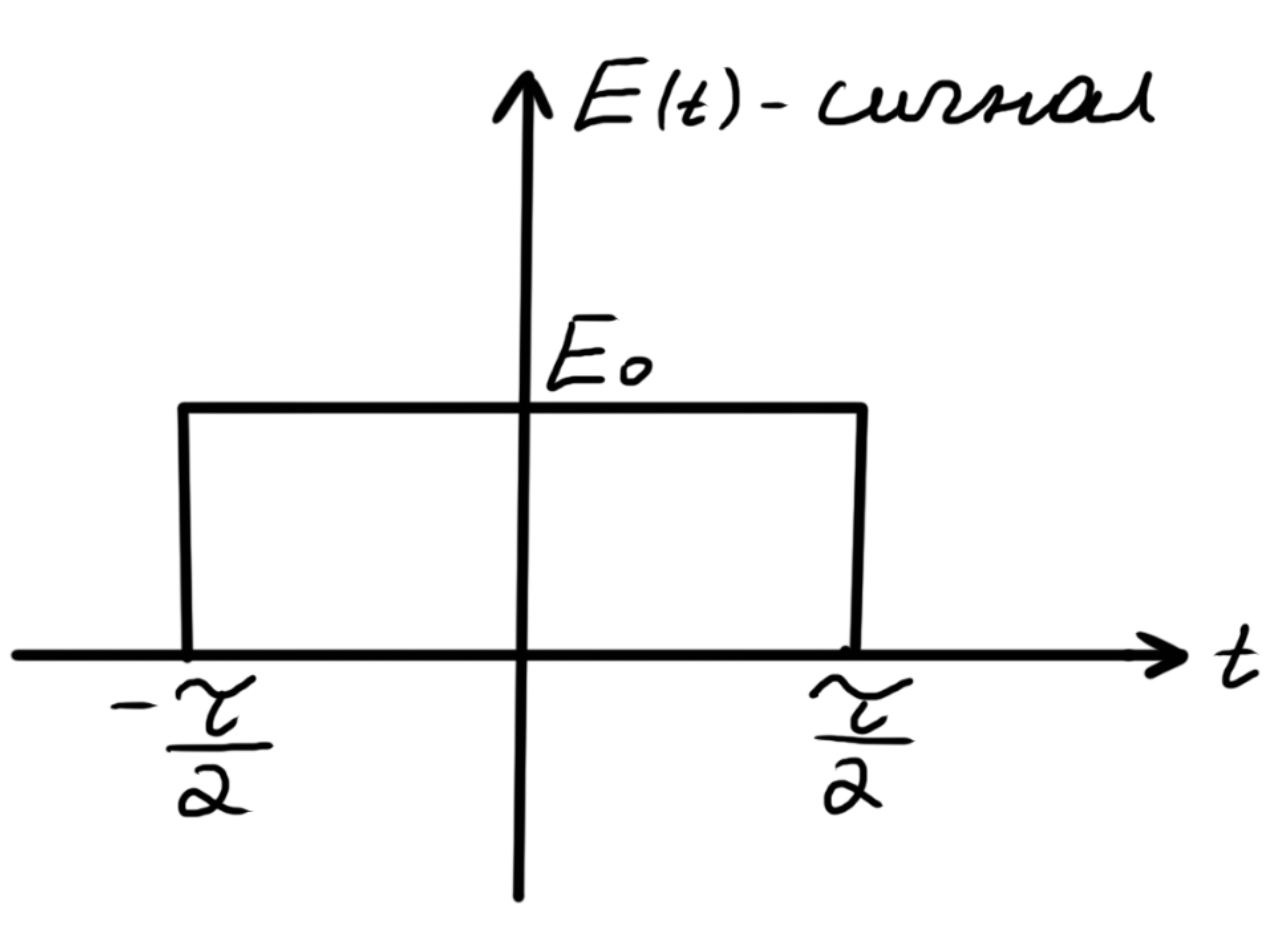
\includegraphics[width=0.3\textwidth]{/Users/vladbelousov/Desktop/Semestr_4-FP-NSU/ЭиО/Лекции_по_дням/image/15.png}
\end{center}

\[ \hat{E}(\omega)= \frac{1}{\sqrt{2 \pi}} \int_{\frac{\tau}{2} }^{-\frac{\tau}{2} } E_0 E^{+ i \omega t} d t = \frac{E_0 \tau}{\sqrt{2 \pi}} \frac{e^{ i \omega \frac{\tau}{2} }- e^{ - i \omega \frac{\tau}{2} }}  {2 i \omega \frac{\tau}{2} }     = \frac{E_0 \tau}{\sqrt{2 \pi}} \mathrm{sinc} ( \frac{\omega \tau}{2} )   \] 

\begin{center}
    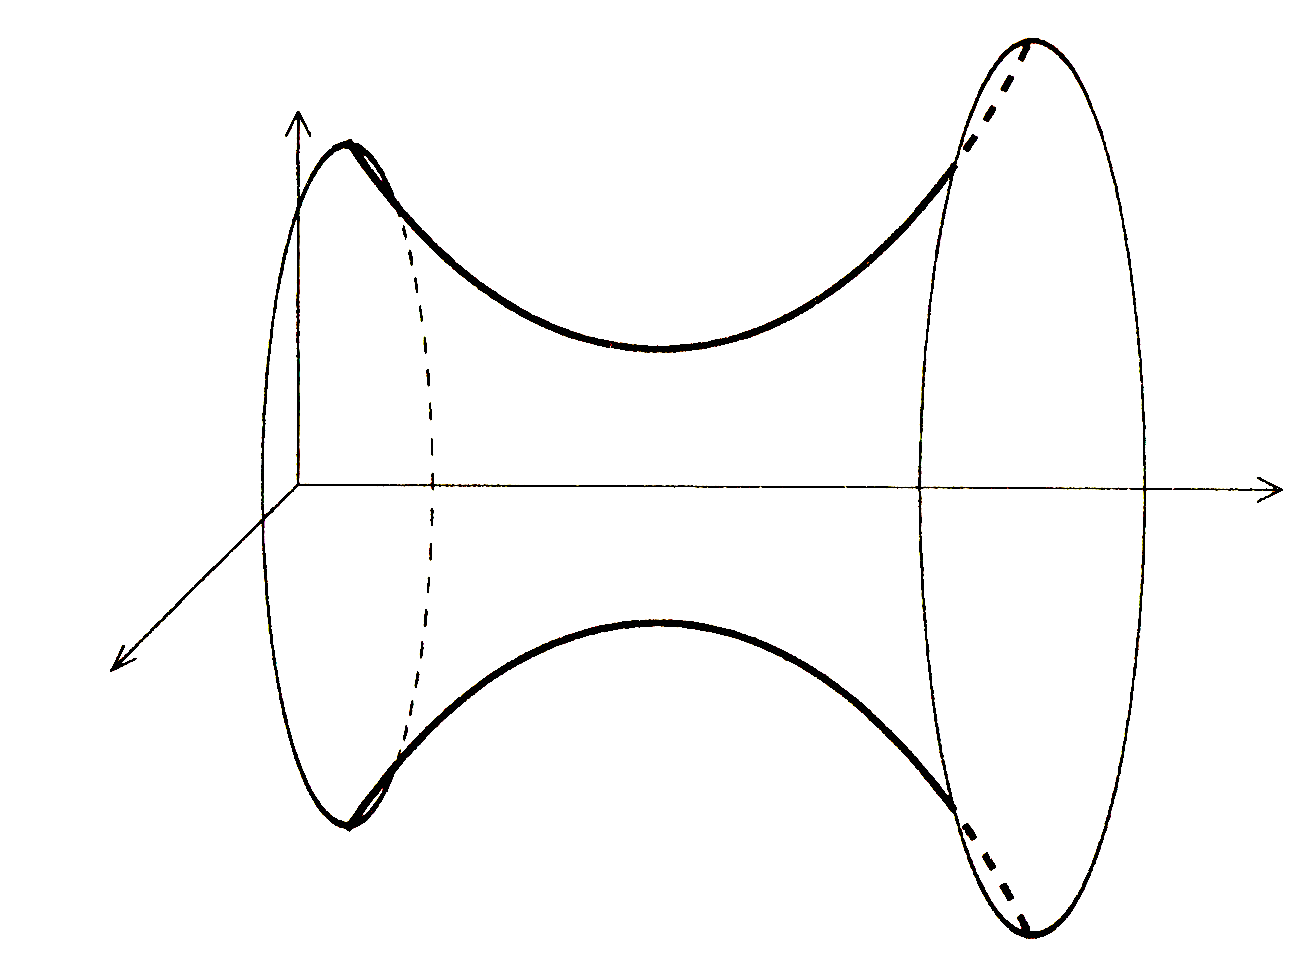
\includegraphics[width=0.5\textwidth]{/Users/vladbelousov/Desktop/Semestr_4-FP-NSU/ЭиО/Лекции_по_дням/image/16.png}
\end{center}

Спектральная плотность энергии = \( |\hat{E } (\omega)| ^2  \) 

\begin{center}
    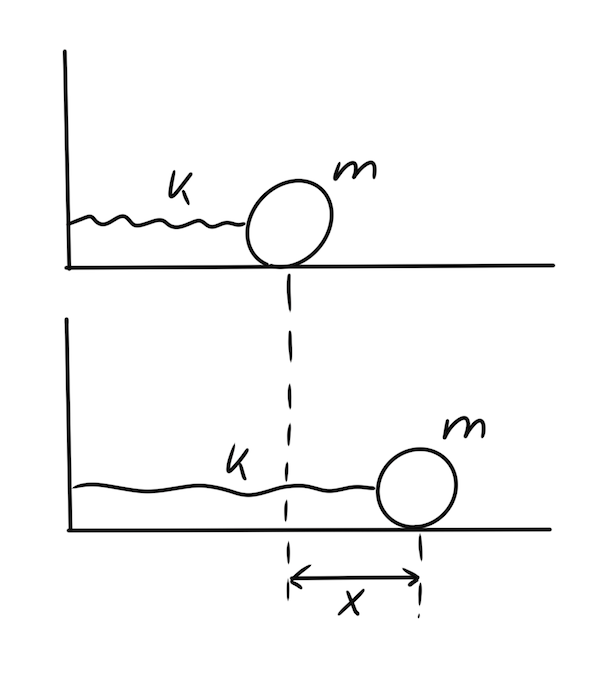
\includegraphics[width=0.5\textwidth]{/Users/vladbelousov/Desktop/Semestr_4-FP-NSU/ЭиО/Лекции_по_дням/image/17.png}
\end{center}

\[ \Delta \omega \sim  \frac{2 \pi}{ \tau} \Rightarrow \Delta \omega \tau \sim \pi - \text{ соотношение неопределенности}     \] 

\[ \tau \to  \infty \Rightarrow \hat{E } \sim  \delta ( \omega)  \] 



2)Спектр синусоидальной волны: 

\[ \begin{aligned}
    E_2 ( t) = \begin{cases}
        E_0 \sin  \omega_0 t , |t| \le \frac{\tau}{2} \\
        0 , |t| > \frac{\tau}{2}
    \end{cases}, 
    \omega_0 = \frac{2 \pi}{\tau} \quad \text{, пусть } \tau= N T , N(\text{целое} ) \gg 1 
\end{aligned} \] 

\begin{center}
    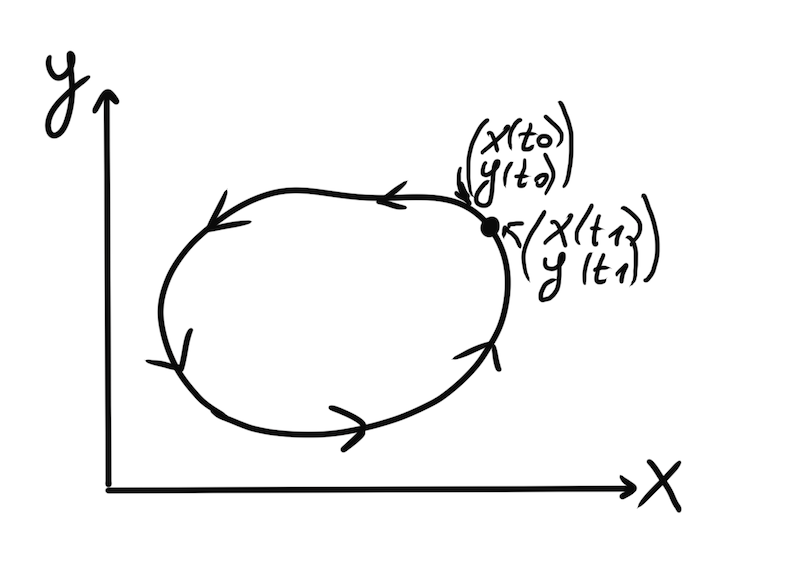
\includegraphics[width=0.5\textwidth]{/Users/vladbelousov/Desktop/Semestr_4-FP-NSU/ЭиО/Лекции_по_дням/image/18.png}
\end{center}


\[ \hat{E_2 } ( \omega) = \frac{1}{ \sqrt{2 \pi}} \int_{-\infty}^{\infty} \frac{ e^{ i \omega_0 t } - e^{- i \omega_0 t} }{2 i} e^{i \omega t} dt  = \frac{1}{2i} \left\{ \frac{E_0 \tau}{\sqrt{2 \pi}}\mathrm{sinc} \left[ (\omega + \omega_0) \frac{\tau}{2}  \right] -    \frac{E_0 \tau}{\sqrt{2 \pi}}\mathrm{sinc} \left[ (\omega - \omega_0) \frac{\tau}{2}  \right]\right\}      \] 

\begin{center}
    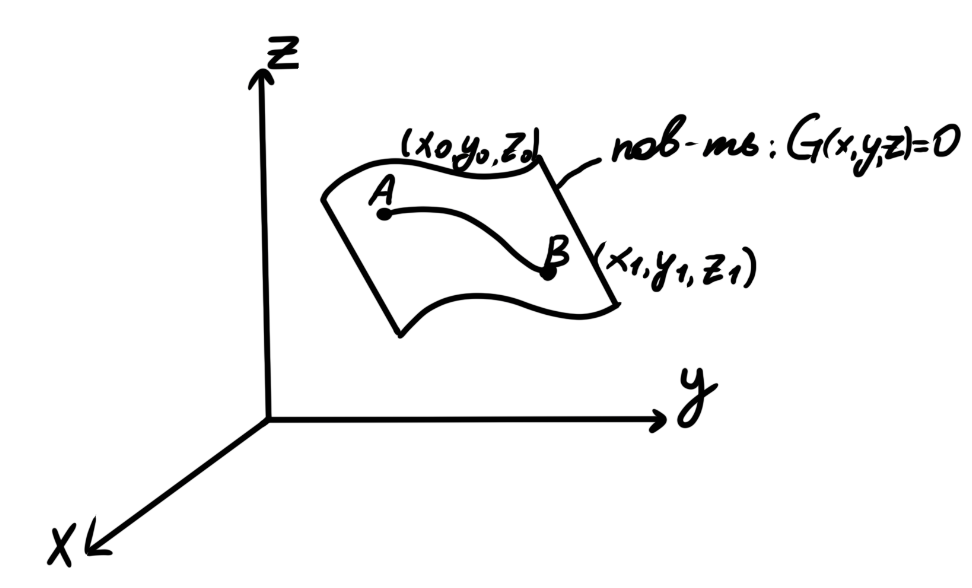
\includegraphics[width=0.45\textwidth]{/Users/vladbelousov/Desktop/Semestr_4-FP-NSU/ЭиО/Лекции_по_дням/image/19.png}
    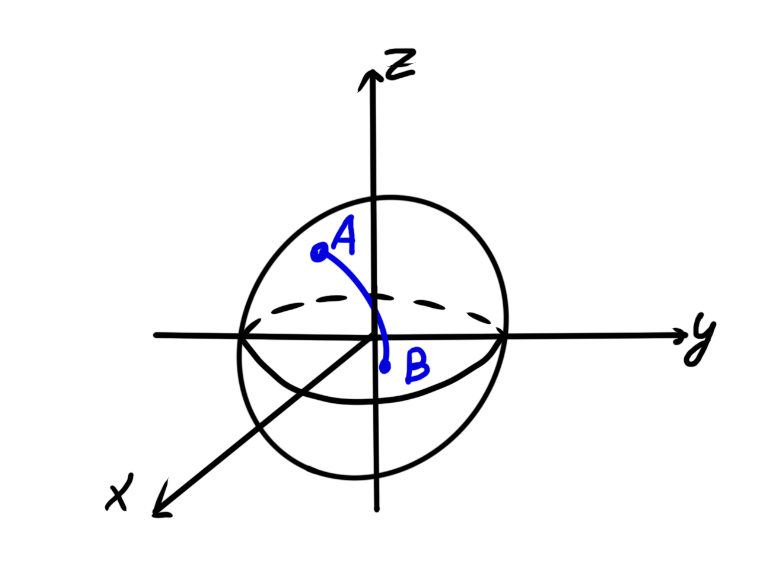
\includegraphics[width=0.45\textwidth]{/Users/vladbelousov/Desktop/Semestr_4-FP-NSU/ЭиО/Лекции_по_дням/image/20.png}
\end{center}

Если \( \frac{\Delta \omega}{\omega_0} \ll 1   \), то такая волна - квазимонохроматическая. 

3) Спектр радиационно затухающего осциллятора:

Механистическая модель атома:

\[ E(t)= \begin{cases}
E_0 e^{ \gamma t} \cos \omega_0 t , t >0\\
0, t < 0
\end{cases} \] 

\[ \gamma = \frac{e ^2 \omega_0 ^2 }{3 m c ^2 } \sim 10 ^9 c^{-1} \quad  \omega_0 \approx 2 \cdot 10^{16} \frac{rad}{c}  \Rightarrow f \sim 3 \cdot 10^8 c^{-1}    \] 

\[ e^{ - \gamma t} = e^{- \frac{t}{\tau} } \Rightarrow \tau \sim \frac{1}{\gamma}      \] 

\begin{center}
    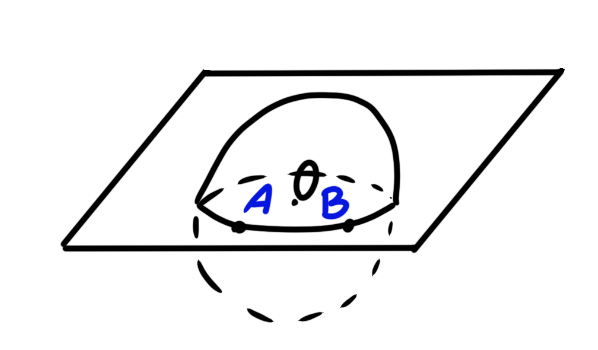
\includegraphics[width=0.5\textwidth]{/Users/vladbelousov/Desktop/Semestr_4-FP-NSU/ЭиО/Лекции_по_дням/image/21.png}
\end{center}

\[ \hat{E} ( \omega ) =\frac{1}{\sqrt{2 \pi}}  \int_{0}^{\infty} E_0 e^{ - \gamma t } \frac{ e^{i \omega_0 t}+ e^{- i \omega_0 t} }{2}  e^{+ i \omega t }   d t     \] 

\[ \hat{E}(\omega) = \frac{E_0}{2 \sqrt{2 \pi}} \left\{ -\frac{1}{- \gamma + i (\omega + \omega_0)}-\frac{1}{- \gamma + i (\omega - \omega_0)}  \right\} = \hat{ f}( \omega + \omega_0) \hat{f}( \omega - \omega_0 )  \]

\[ \lvert \hat{f}(\omega- \omega_0 )   \rvert ^2 = \frac{E_0 ^2 }{8 \pi} \] 

\begin{center}
    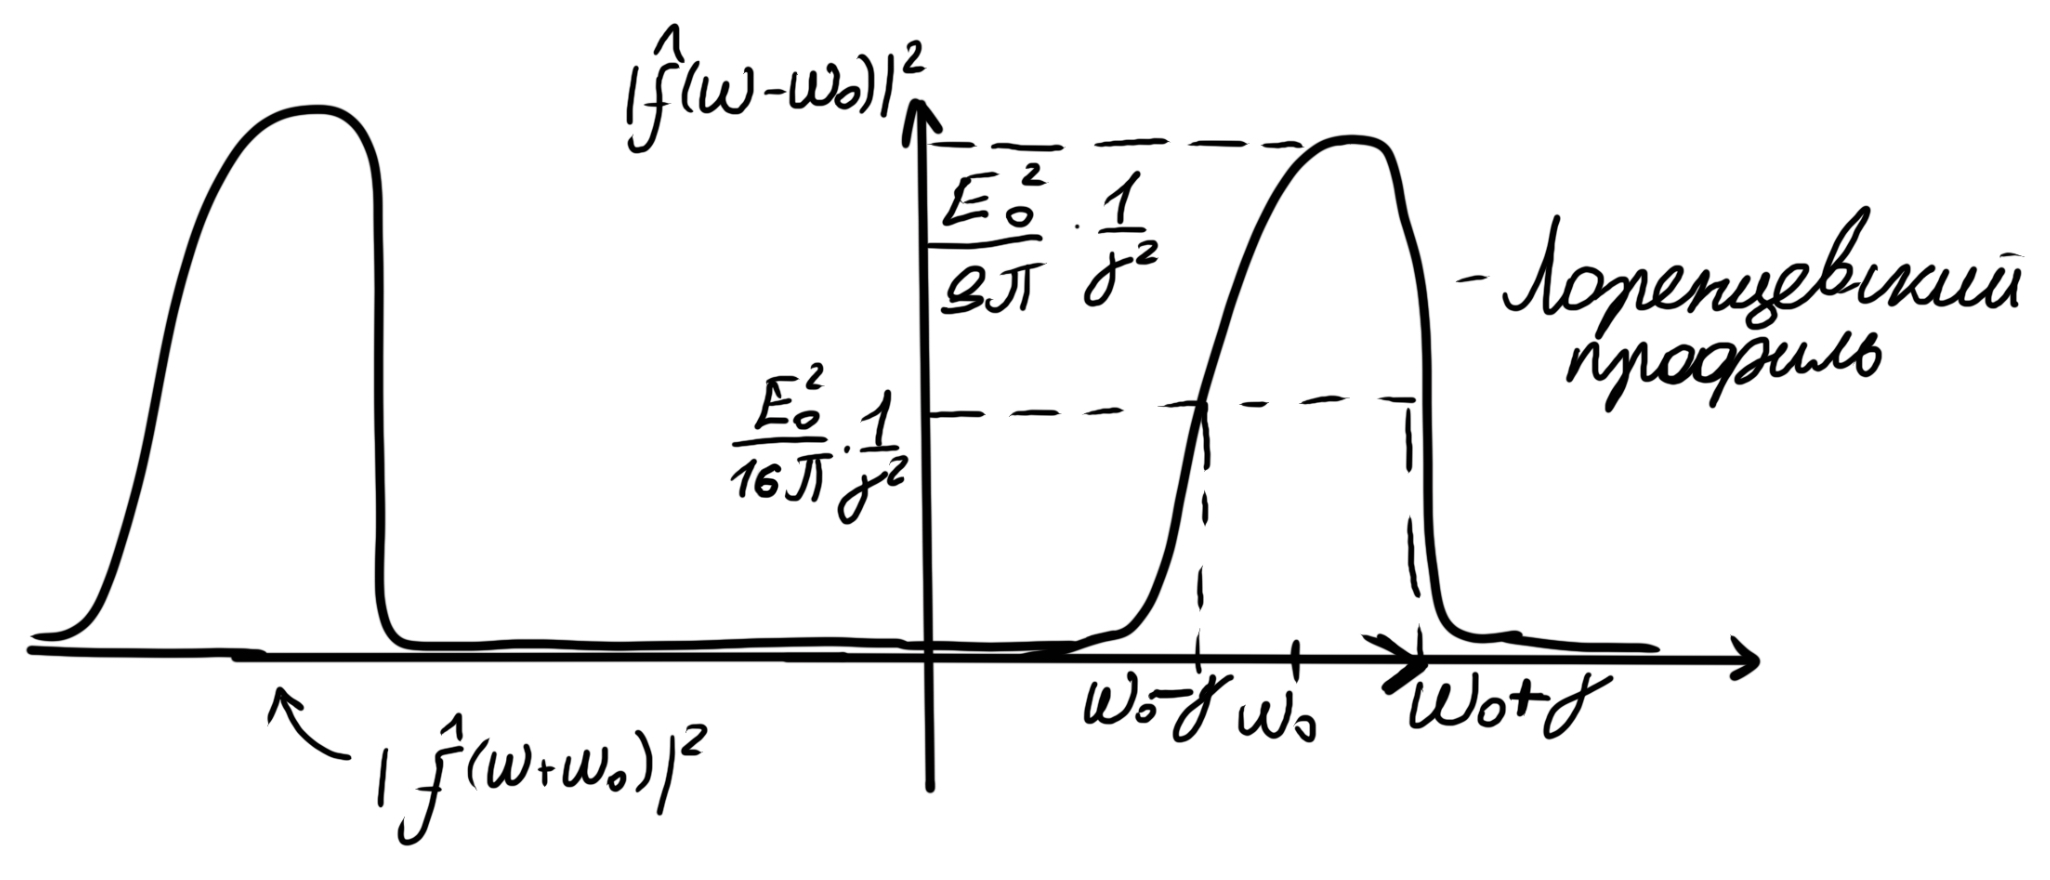
\includegraphics[width=0.55\textwidth]{/Users/vladbelousov/Desktop/Semestr_4-FP-NSU/ЭиО/Лекции_по_дням/image/22.png}
\end{center}

\[ \Delta \omega \sim  2 \gamma - \text{ширина спектра}  \] 

\[ \Delta \omega \underbrace{\Delta t}_{\sim  \tau}  \sim 2 \gamma \frac{1}{\gamma} \sim 2   \] 

\[ |\hat{E} ( \omega ) | ^2 = |\hat{f}(\omega + \omega_0) | ^2 + |\hat{f}(\omega - \omega_0) | ^2 + \cancel{\text{поправка}}  \] 

Поправка  мала, если \( 10^9 c^{-1} \sim\Delta \omega \ll \omega_0 \sim 2 \cdot 10^{16} \frac{rad}{c}  \) 

4) Спектр гауссовой функции : \( f(x) = E_0 e^{ -\alpha x ^2} \quad  \hat{f}( x) = \frac{1}{\sqrt{2 \pi}} \int_{-\infty}^{\infty}   f( x) e^{- i kx }dx =     \) 

\[ \frac{1}{\sqrt{2 \pi}}E_0 \int_{-\infty}^{\infty} e^{- \alpha x ^2 - ikx } dx ; -\alpha x ^2 - ikx = -\alpha \left( x ^2 + 2x \frac{ik}{2 \alpha} - \frac{k ^2}{4 \alpha ^2}   \right) - \frac{k ^2}{4\alpha} =  - \alpha \left( x + \frac{ik}{2\alpha} \right) ^2 - \frac{k ^2}{4\alpha}    \] 

\begin{center}
    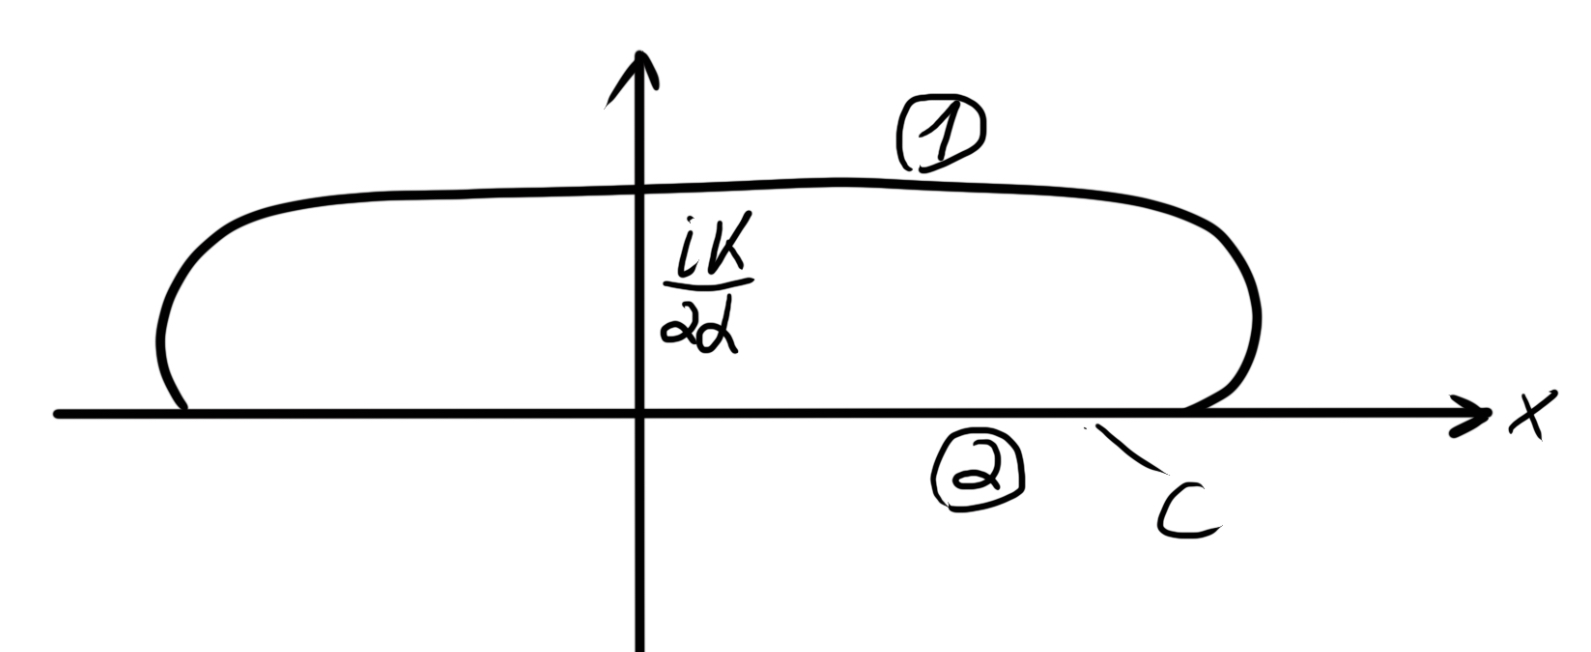
\includegraphics[width=0.4\textwidth]{/Users/vladbelousov/Desktop/Semestr_4-FP-NSU/ЭиО/Лекции_по_дням/image/23.png}
\end{center}

\[  \int_{C} e^{- \alpha z ^2 }dz = 0 = \int_{1} + \int_{ 2} \Rightarrow \int_{1} = \int _{-2}  \] 

\[ \int_{-\infty}^{\infty} e^{-\alpha z ^2 } dz = \int_{-\infty}^{\infty} e^{ - \alpha x ^2 } dx = \sqrt{\frac{\pi}{\alpha} }    \] 

\[ \hat{f} (k) = \frac{ E_0}{\sqrt{2 \pi}} \sqrt{\frac{\pi}{\alpha}} e^{- \frac{k ^2}{4 \alpha} }    \]

\begin{center}
    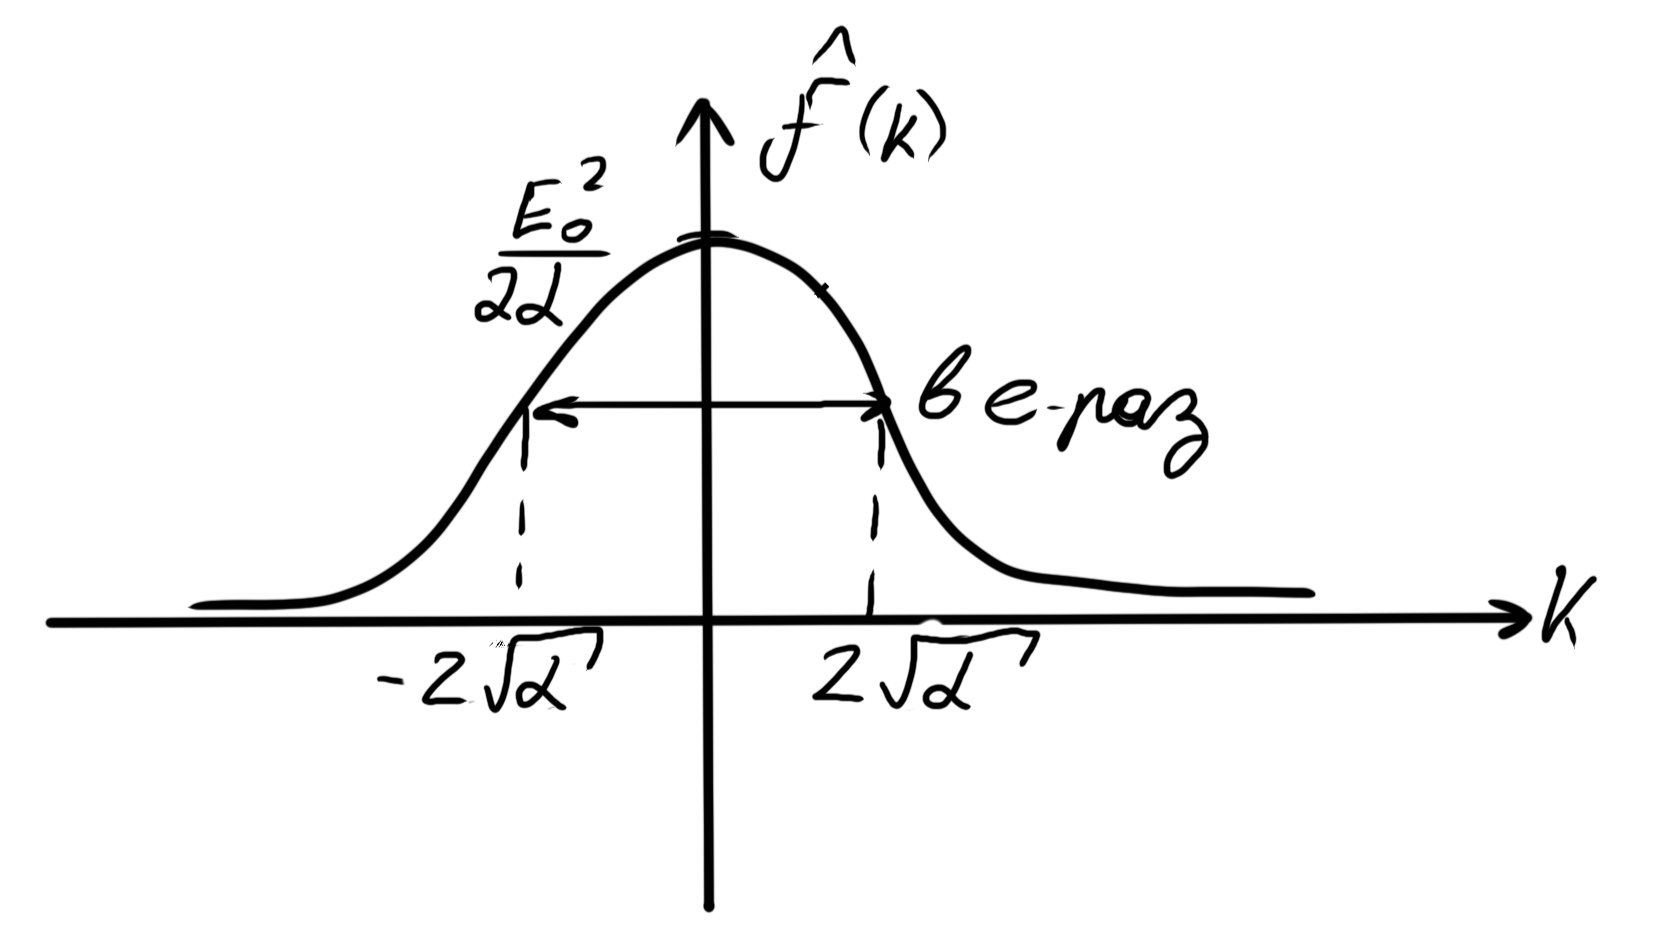
\includegraphics[width=0.45\textwidth]{/Users/vladbelousov/Desktop/Semestr_4-FP-NSU/ЭиО/Лекции_по_дням/image/24.png}
    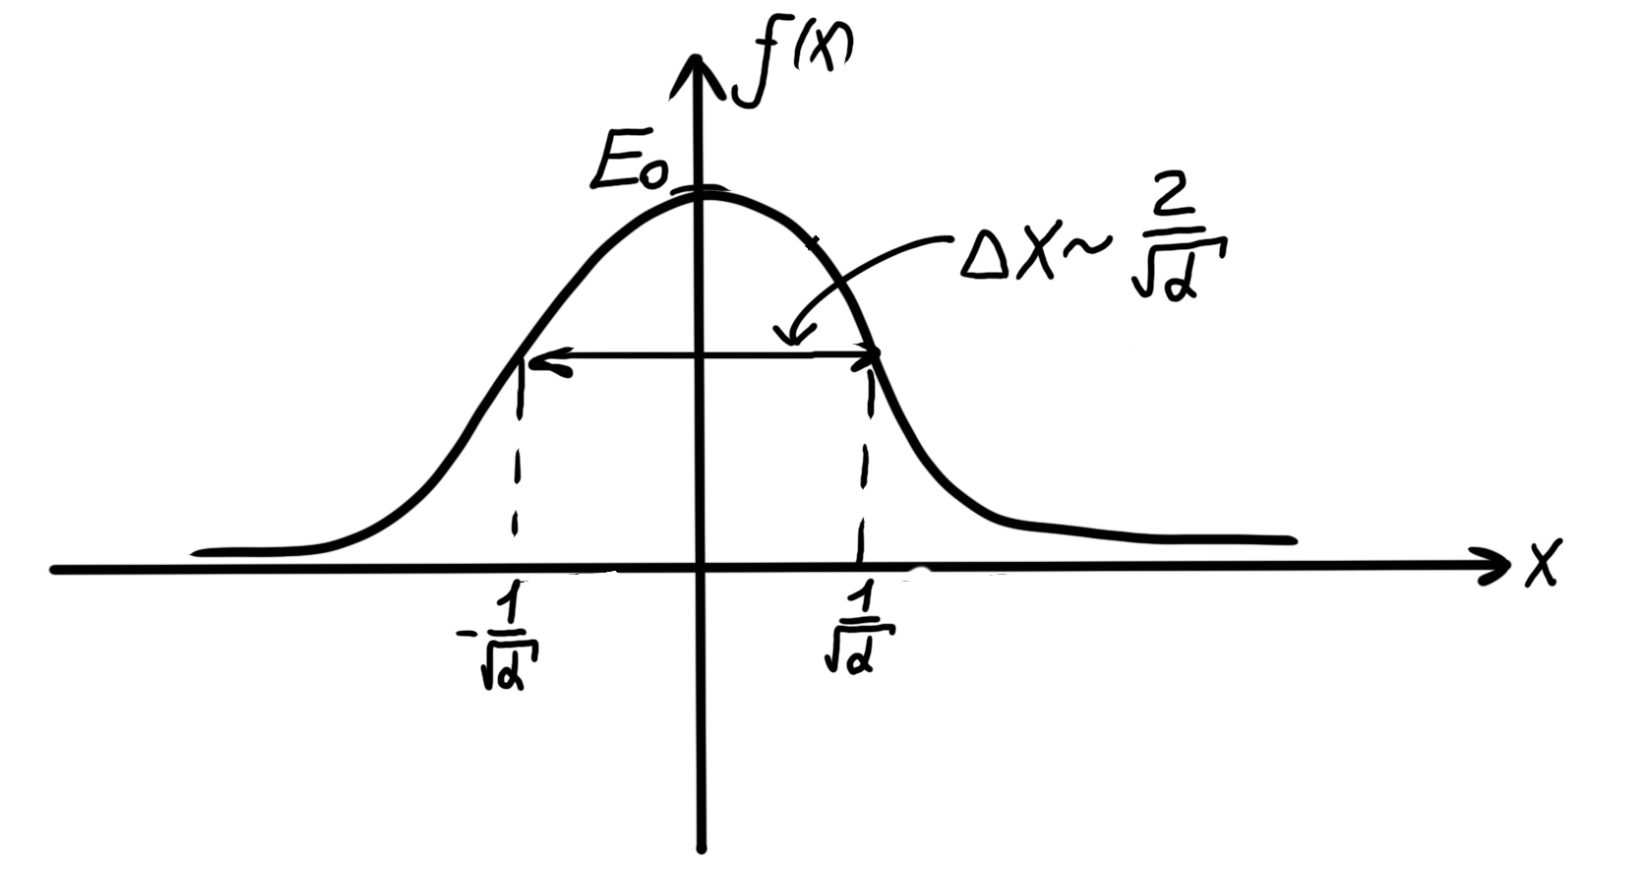
\includegraphics[width=0.45\textwidth]{/Users/vladbelousov/Desktop/Semestr_4-FP-NSU/ЭиО/Лекции_по_дням/image/25.png}
\end{center}


\[\begin{aligned}
    \begin{array}{l}
        \Delta k \sim  4 \sqrt{\alpha} \\
        \Delta x \sim \frac{2}{\sqrt{\alpha}}
    \end{array}
    \Rightarrow 
    \Delta k \Delta x \sim 8 \sim \pi 
\end{aligned} \] 

5) Модулированный гауссиан: \( E(x) = E_0 e^{ - \alpha x ^2} \cos k_0x \) 

\section{Преобразование Фурье функции четырех переменных (x,y,z,t). Уравнения Максвелла в Фурье преобразованиия}

\[ f(x,y,z,t) = \frac{1}{\sqrt{ 2 \pi} ^4} \iiiint \hat{f}(k_x,k_y,k_z,k_t) e^{  i k_x x } e^{ i k_y y } e^{  i k_z z } e^{ - i \omega t } dk_x dk_y dk_z dk_t    \] 

\[ f( \vec{r},t) = \frac{1}{(2 \pi) ^2 } \iiiint \hat{f} ( \vec{k}, \omega) e^{ i( \vec{k},\vec{r})- i\omega t} d^3 k d \omega    \]  

\[ \frac{\partial f( \vec{r},t)}{\partial t} = \frac{1}{( 2 \pi ) ^2} \iiiint \hat{f}(\vec{k}, \omega) ( - i \omega) e^{i \vec{k}\vec{r} - i \omega t} d^3 k d \omega \quad \frac{\partial f}{\partial t}  \risingdotseq   - i \omega \hat{f}( \vec{k}, \omega)    \] 

\[ \frac{\partial f (\vec{r},t)}{\partial x} \risingdotseq i k_x \hat{f}( \vec{k}, \omega) \]

\[ \mathrm{div} \hat{\vec{D}}(\vec{r},t) = \frac{\partial \hat{\vec{D_x}}}{\partial x} + \frac{\partial \hat{\vec{D_y}}}{\partial y} + \frac{\partial \hat{\vec{D_z}}}{\partial z} \risingdotseq i k_x \hat{D_x}(\vec{k}, \omega) + i k_y \hat{D_y}(\vec{k}, \omega) + i k_z \hat{D_z}(\vec{k}, \omega)  = i (\vec{k},\hat{\vec{D}}(\vec{r}, \omega) ) \] 

\[ \mathrm{rot}\hat{\vec{E}}  = [\nabla \times  \hat{\vec{E}} ] = \frac{1}{( 2 \pi ) ^2 } \iiiint \underbrace{\left[ (\nabla \times  \hat{\vec{E}} (\vec{k}, \omega)e^{i (\vec{k}\vec{r}) }   ) \right]}_{\nabla e^{i (\vec{k }, \vec{r })}   \times \vec{E } (\vec{k },\omega) }   e^{- i \omega t } d ^3 d \omega  =      \] 

\begin{center}
    Где \(\nabla e^{i (\vec{k }, \vec{r })} = \vec{e_x }i k_xe^{(i (\vec{k }, \vec{r }))}+ \vec{e_y } i k_y e^{(i (\vec{k }, \vec{r }))} + \vec{e_z } i k_z e^{(i (\vec{k }, \vec{r }))}= i\vec{k } e ^{ i ( \vec{k } , \vec{r})} \)    
\end{center}


\[= \frac{1}{( 2 \pi) ^2 } \iiiint \left[ i \vec{k} \times  \hat{\vec{E }}( \vec{k }, \omega)  \right] e^{i(\vec{k}, \vec{r})- i \omega t} d ^3 k d \omega \] 

\[ \mathrm{rot} \vec{ E }  \risingdotseq i \left[ \vec{k} \times \hat{\vec{E}}(\vec{k}, \omega) \right]   \] 
 
\[ 
\begin{cases}
        \displaystyle \mathrm{rot} \vec{ E } = - \frac{1}{c} \frac{ \partial \vec{B}}{ \partial t} \risingdotseq i \left[ \vec{k } \times \hat{\vec{E}} ( \vec{k }, \omega)  \right] = \frac{i \omega}{c} \hat{\vec{B } } ( \vec{k }, \omega)     \\
        \displaystyle \mathrm{rot} \vec{H} = \frac{ 4 \pi }{ c} \vec{j } + \frac{1}{ c  }  \frac{ \partial \vec{ D } }{ \partial t } \risingdotseq  i \left[ \vec{k } \times \hat{\vec{H}} ( \vec{k }, \omega) \right] = \frac{  4 \pi }{ c } \hat{\vec{j}} ( \vec{k }, \omega)  - \frac{ i \omega }{c } \hat{ \vec{D} } ( \vec{k }, \omega)        \\
        \displaystyle \mathrm{div} \vec{D } = 4 \pi \rho \risingdotseq i ( \vec{k }, \hat{\vec{D}} ( \vec{k }, \omega) ) = 4 \pi \hat{\rho}  ( \vec{k }, \omega)   \\
        \displaystyle \mathrm{div} \vec{B} = 0 \Rightarrow (\vec{k },\hat{\vec{B}} ( \vec{k }, \omega)) = 0    \\
\end{cases}
\] 

В системе слева это уравнения Максвелла, а справа преобразование Фурье уравнений Максвелла.


\[ \frac{ \partial \rho }{ \partial t } + \mathrm{ \div  } \vec{ j }  = 0 \risingdotseq - i \omega \hat{ \rho } ( \vec{k }, \omega) + i ( \vec{k }, \hat{\vec{j}} ( \vec{k }, \omega) ) = 0      \] 

Если \( \vec{B} = \mu \vec{H } , \vec{D } = \varepsilon \vec{ E } , \varepsilon , \mu  - \mathrm{const}   \)

\[ \underset{a}{\vec{k}} \times \left[ \underset{b}{\vec{k} }\times \underset{c}{\vec{E}}  \right] = \frac{\omega \mu}{c }  \left( - \frac{\omega}{ c } \varepsilon \hat{\vec{E}}  \right)
\] 
\( \quad \quad \quad \quad \quad \quad \quad \quad \quad \quad \quad \quad \quad \quad || \) 

\[ \vec{k } \underbrace{( \vec{k }, \hat{\vec{E }})}_{=0} - \hat{ \vec{ E } } k ^2 = - \frac{\varepsilon \mu }{c ^2 } \omega ^2 \hat{\vec{E }} \Rightarrow k ^2 = \frac{ \omega ^2 }{\left( \frac{c}{\sqrt{\varepsilon \mu}}      \right) ^2} = \frac{\omega ^2 }{v ^2 _{\text{в} } }       \] 


%%-------------------------------%%

% Закрытие документа, если файл компилируется отдельно
\ifdefined\mainfile
    % Если это основной файл, не нужно заканчивать документ
\else
    \end{document}
\fi

